\protect\hyperlink{main-nav}{≡} \protect\hyperlink{close-nav}{×}

\hypertarget{section-2.7-optimization}{%
\section{Section 2.7: Optimization}\label{section-2.7-optimization}}

In theory and applications, we often want to maximize or minimize some
quantity. An engineer may want to maximize the speed of a new computer
or minimize the heat produced by an appliance. A manufacturer may want
to maximize profits and market share or minimize waste. A student may
want to maximize a grade in calculus or minimize the hours of study
needed to earn a particular grade.

Without calculus, we only know how to find the optimum points in a few
specific examples (for example, we know how to find the vertex of a
parabola). But what if we need to optimize an unfamiliar function?

The best way we have without calculus is to examine the graph of the
function, perhaps using technology. But our view depends on the viewing
window we choose -- we might miss something important. In addition,
we'll probably only get an approximation this way. (In some cases, that
will be good enough.)

Calculus provides ways of drastically narrowing the number of points we
need to examine to find the exact locations of maximums and minimums,
while at the same time ensuring that we haven't missed anything
important.

To view this video please enable JavaScript, and consider upgrading to a
web browser that \href{http://videojs.com/html5-video-support/}{supports
HTML5 video}

\hypertarget{local-maxima-and-minima}{%
\subsection{Local Maxima and Minima}\label{local-maxima-and-minima}}

Before we examine how calculus can help us find maximums and minimums,
we need to define the concepts we will develop and use.

\hypertarget{definitions-local-maxima-and-minima}{%
\paragraph{Definitions (Local Maxima and
Minima)}\label{definitions-local-maxima-and-minima}}

\textbackslash{}(f(x)\textbackslash{}) has a \textbf{local maximum} at
\textbackslash{}(x=a\textbackslash{}) if \textbackslash{}(f(a)
\textbackslash{}geq f(x)\textbackslash{}) for all
\textbackslash{}(x\textbackslash{}) near
\textbackslash{}(a\textbackslash{}).

\textbackslash{}(f(x)\textbackslash{}) has a \textbf{local minimum} at
\textbackslash{}(x=a\textbackslash{}) if \textbackslash{}(f(a)
\textbackslash{}leq f(x)\textbackslash{}) for all
\textbackslash{}(x\textbackslash{}) near
\textbackslash{}(a\textbackslash{}).

\textbackslash{}(f(x)\textbackslash{}) has a \textbf{local extreme} at
\textbackslash{}(x=a\textbackslash{}) if
\textbackslash{}(f(a)\textbackslash{}) is a \textbf{local maximum or
minimum}.

The plurals of these are maxima and minima. We often simply say "max" or
"min;" it saves a lot of syllables.

Some books say "relative" instead of "local."

The process of finding maxima or minima is called \textbf{optimization}.

A point is a local max (or min) if it is higher (lower) than all the
\textbf{nearby points}. These points come from the shape of the graph.

\hypertarget{definitions-global-maxima-and-minima}{%
\paragraph{Definitions (Global Maxima and
Minima)}\label{definitions-global-maxima-and-minima}}

\textbackslash{}(f(x)\textbackslash{}) has a \textbf{global maximum} at
\textbackslash{}(x=a\textbackslash{}) if \textbackslash{}(f(a)
\textbackslash{}geq f(x)\textbackslash{}) for all
\textbackslash{}(x\textbackslash{}) in the domain of
\textbackslash{}(f(x)\textbackslash{}).

\textbackslash{}(f(x)\textbackslash{}) has a \textbf{global minimum} at
\textbackslash{}(x=a\textbackslash{}) if \textbackslash{}(f(a)
\textbackslash{}leq f(x)\textbackslash{}) for all
\textbackslash{}(x\textbackslash{}) in the domain of
\textbackslash{}(f(x)\textbackslash{}).

\textbackslash{}(f(x)\textbackslash{}) has a \textbf{global extreme} at
\textbackslash{}(x=a\textbackslash{}) if
\textbackslash{}(f(a)\textbackslash{}) is a \textbf{global maximum or
minimum}.

Some books say "absolute" instead of "global."

A point is a global max (or min) if it is higher (lower) than every
point on the graph. These points come from the shape of the graph
\textbf{and} the window through which we view the graph.

The local and global extremes of the function in Figure 1 are labeled.
You should notice that every global extreme is also a local extreme, but
there are local extremes that are not global extremes.

\begin{figure}
\centering
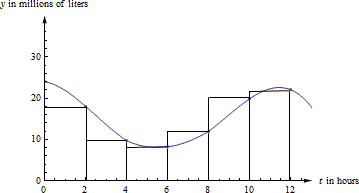
\includegraphics{images/image056.png}
\caption{Figure 1}
\end{figure}

If \textbackslash{}(h(x)\textbackslash{}) is the height of the earth
above sea level at the location \textbackslash{}(x\textbackslash{}),
then the global maximum of \textbackslash{}(h\textbackslash{}) is
\textbackslash{}(h\textbackslash{})(summit of Mt. Everest) = 29,028
feet. The local maximum of \textbackslash{}(h\textbackslash{}) for the
United States is \textbackslash{}(h\textbackslash{})(summit of Mt.
McKinley) = 20,320 feet. The local minimum of
\textbackslash{}(h\textbackslash{}) for the United States is
\textbackslash{}(h\textbackslash{})(Death Valley) = -282 feet.

\hypertarget{example-1}{%
\paragraph{Example 1}\label{example-1}}

The table shows the annual calculus enrollments at a large university.
Which years had local maximum or minimum calculus enrollments? What were
the global maximum and minimum enrollments in calculus?

\begin{longtable}[]{@{}llllllllllll@{}}
\toprule
\endhead
Year & 2000 & 2001 & 2002 & 2003 & 2004 & 2005 & 2006 & 2007 & 2008 &
2009 & 2010\tabularnewline
Enrollment & 1257 & 1324 & 1378 & 1336 & 1389 & 1450 & 1523 & 1582 &
1567 & 1545 & 1571\tabularnewline
\bottomrule
\end{longtable}

There were local maxima in 2002 and 2007; the global maximum was 1582
students in 2007. There were local minima in 2003 and 2009; the global
minimum was 1257 students in 2000. We choose not to think of 2000 as a
local minimum or 2010 as a local maximum; however, some books would
include the endpoints. We are allowed to have a global maximum or global
minimum at an endpoint.

To view this video please enable JavaScript, and consider upgrading to a
web browser that \href{http://videojs.com/html5-video-support/}{supports
HTML5 video}

\hypertarget{finding-maxima-and-minima-of-a-function}{%
\subsection{Finding Maxima and Minima of a
Function}\label{finding-maxima-and-minima-of-a-function}}

What must the tangent line look like at a local max or min? Look at
these two graphs again -- you'll see that at all the extreme points, the
tangent line is horizontal (so \textbackslash{}(f' =
0\textbackslash{})). There is one cusp in the blue graph -- the tangent
line is vertical there (so \textbackslash{}(f'\textbackslash{}) is
undefined).

\begin{figure}
\centering
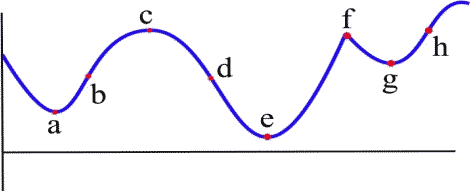
\includegraphics{images/image053.png}
\caption{}
\end{figure}

That gives us the clue how to find extreme values.

\hypertarget{definitions}{%
\paragraph{Definitions}\label{definitions}}

A \textbf{critical number} for a function
\textbackslash{}(f\textbackslash{}) is a value \textbackslash{}(x =
a\textbackslash{}) in the domain of \textbackslash{}(f\textbackslash{})
where either \textbackslash{}(f'(a) = 0\textbackslash{}) or
\textbackslash{}(f'(a)\textbackslash{}) is undefined.

A \textbf{critical point} for a function f is a point (a, f(a)) where a
is a critical number of f.

\textbf{A local max or min of f can only occur at a critical point.}

\hypertarget{example-2}{%
\paragraph{Example 2}\label{example-2}}

Find the critical points of \textbackslash{}(f(x) = x\^{}3 - 6x\^{}2 +
9x + 2\textbackslash{}).

A critical number of \textbackslash{}(f\textbackslash{}) can occur only
where \textbackslash{}(f'(x) = 0\textbackslash{}) or where
\textbackslash{}(f'\textbackslash{}) does not exist.

\textbackslash{}{[}f '(x) = 3x\^{}2 - 12x + 9 = 3(x\^{}2 - 4x + 3) = 3(x
- 1)(x - 3)\textbackslash{}{]} So \textbackslash{}(f'(x) =
0\textbackslash{}) at \textbackslash{}(x = 1\textbackslash{}) and
\textbackslash{}(x = 3\textbackslash{}) (and no other values of
\textbackslash{}( x \textbackslash{})). There are no places where
\textbackslash{}(f'\textbackslash{}) is undefined.

The critical numbers are \textbackslash{}(x = 1\textbackslash{}) and
\textbackslash{}(x= 3\textbackslash{}). So the critical points are (1,
6) and (3, 2).

These are the only possible locations of local extremes of
\textbackslash{}(f\textbackslash{}). We haven't discussed yet how to
tell whether either of these points is actually a local extreme of
\textbackslash{}(f\textbackslash{}), or which kind it might be. But we
can be certain that no other point is a local extreme.

The graph of \textbackslash{}(f\textbackslash{}) below shows that
\textbackslash{}((1, f(1) ) = (1, 6)\textbackslash{}) is a local maximum
and \textbackslash{}((3, f(3) ) = (3, 2)\textbackslash{}) is a local
minimum. This function does not have a global maximum or minimum.

\begin{figure}
\centering
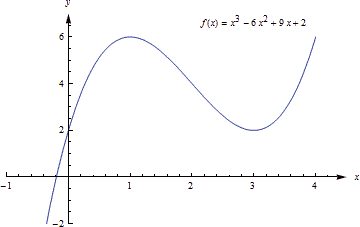
\includegraphics{images/image058.png}
\caption{}
\end{figure}

\hypertarget{example-3}{%
\paragraph{Example 3}\label{example-3}}

Find all local extremes of \textbackslash{}(f(x) =
x\^{}3\textbackslash{}).

\textbackslash{}(f(x) = x\^{}3\textbackslash{}) is differentiable for
all \textbackslash{}(x\textbackslash{}), and \textbackslash{}(f'(x) =
3x\^{}2\textbackslash{}). The only place where \textbackslash{}(f'(x) =
0\textbackslash{}) is at \textbackslash{}(x = 0\textbackslash{}), so the
only candidate is the critical point (0,0).

If \textbackslash{}(x \textbackslash{}gt 0\textbackslash{}) then
\textbackslash{}(f(x) = x\^{}3 \textbackslash{}gt 0 =
f(0)\textbackslash{}), so \textbackslash{}(f(0)\textbackslash{}) is not
a local maximum.

Similarly, if \textbackslash{}(x \textbackslash{}lt 0\textbackslash{})
then \textbackslash{}(f(x) = x\^{}3 \textbackslash{}lt 0 =
f(0)\textbackslash{}) so \textbackslash{}(f(0)\textbackslash{}) is not a
local minimum.

The critical point (0,0) is the only candidate to be a local extreme of
\textbackslash{}(f\textbackslash{}), and, based on the graph, this
candidate did not turn out to be a local extreme of
\textbackslash{}(f\textbackslash{}). The function \textbackslash{}(f(x)
= x\^{}3\textbackslash{}) does not have any local extremes.

\begin{figure}
\centering
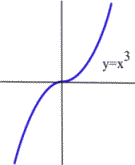
\includegraphics{images/image059.png}
\caption{}
\end{figure}

Remember this example! It is not enough to find the critical points --
we can only say that \textbackslash{}(f\textbackslash{}) \emph{might}
have a local extreme at the critical points.

\hypertarget{first-and-second-derivative-tests}{%
\subsection{First and Second Derivative
Tests}\label{first-and-second-derivative-tests}}

\hypertarget{is-that-critical-point-a-maximum-or-minimum-or-neither}{%
\subsubsection{Is that critical point a Maximum or Minimum (or
Neither)?}\label{is-that-critical-point-a-maximum-or-minimum-or-neither}}

Once we have found the critical points of
\textbackslash{}(f\textbackslash{}), we still have the problem of
determining whether these points are maxima, minima or neither.

All of the graphs in the figure below have a critical point at (2, 3).
It is clear from the graphs that the point (2,3) is a local maximum in
(a) and (d), (2,3) is a local minimum in (b) and (e), and (2,3) is not a
local extreme in (c) and (f).

\begin{figure}
\centering
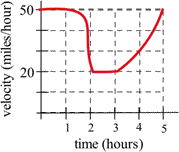
\includegraphics{images/image060.png}
\caption{}
\end{figure}

The critical numbers only give the \emph{possible} locations of
extremes, and some critical numbers are not the locations of extremes.
The critical numbers are the \emph{candidates} for the locations of
maxima and minima.

\hypertarget{f-and-extreme-values-of-f}{%
\subsubsection{\textbackslash{}(f'\textbackslash{}) and Extreme Values
of
\textbackslash{}(f\textbackslash{})}\label{f-and-extreme-values-of-f}}

Four possible shapes of graphs are shown here -- in each graph, the
point marked by an arrow is a critical point, where
\textbackslash{}(f'(x) = 0\textbackslash{}). What happens to the
derivative near the critical point?

\begin{figure}
\centering
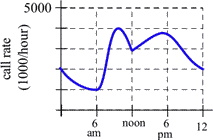
\includegraphics{images/image061.png}
\caption{}
\end{figure}

At a local max, such as in the graph on the left, the function increases
on the left of the local max, then decreases on the right. The
derivative is first positive, then negative at a local max. At a local
min, the function decreases to the left and increases to the right, so
the derivative is first negative, then positive. When there isn't a
local extreme, the function continues to increase (or decrease) right
past the critical point -- the derivative doesn't change sign.

\hypertarget{the-first-derivative-test-for-extremes}{%
\paragraph{The First Derivative Test for
Extremes}\label{the-first-derivative-test-for-extremes}}

Find the critical points of f.

For each critical number c, examine the sign of f' to the left and to
the right of c. What happens to the sign as you move from left to right?

\begin{itemize}
\tightlist
\item
  If \textbackslash{}(f'(x)\textbackslash{}) \textbf{changes from
  positive to negative} at \textbackslash{}(x = c\textbackslash{}), then
  \textbackslash{}(f\textbackslash{}) has a \textbf{local maximum} at
  \textbackslash{}((c, f(c))\textbackslash{}).
\item
  If \textbackslash{}(f'(x)\textbackslash{}) \textbf{changes from
  negative to positive} at \textbackslash{}(x = c\textbackslash{}), then
  \textbackslash{}(f\textbackslash{}) has a \textbf{local minimum} at
  \textbackslash{}((c, f(c))\textbackslash{}).
\item
  If \textbackslash{}(f'(x)\textbackslash{}) \textbf{does not change
  sign} at \textbackslash{}(x = c\textbackslash{}), then
  \textbackslash{}((c, f(c))\textbackslash{}) is \textbf{neither} a
  local maximum nor a local minimum.
\end{itemize}

To view this video please enable JavaScript, and consider upgrading to a
web browser that \href{http://videojs.com/html5-video-support/}{supports
HTML5 video}

\hypertarget{example-4}{%
\paragraph{Example 4}\label{example-4}}

Find the critical points of \textbackslash{}(f(x) = x\^{}3 - 6x\^{}2 +
9x + 2\textbackslash{}) and classify them as local max, local min, or
neither.

We already found the critical points; they are (1, 6) and (3, 2).

Now we can use the first derivative test to classify each. Recall that
\textbackslash{}(f'(x) = 3x\^{}2 - 12x + 9 = 3(x\^{}2 - 4x + 3) = 3(x -
1)(x - 3)\textbackslash{}). The factored form is easiest to work with
here, so let's use that.

At (1, 6) we could choose a number slightly less than 1 to plug into the
formula for \textbackslash{}(f'\textbackslash{}) -- perhaps use
\textbackslash{}(x = 0\textbackslash{}), or \textbackslash{}(x =
0.9\textbackslash{}). Then we could examine its sign. But we don't care
about the numerical value, all we are interested in is its sign. And for
that, we don't have to do any plugging in:

\begin{itemize}
\tightlist
\item
  If \textbackslash{}(x\textbackslash{}) is a little less than 1, then
  \textbackslash{}(x-1\textbackslash{}) is negative, and
  \textbackslash{}(x-3\textbackslash{}) is negative. So
  \textbackslash{}(f' = 3(x - 1)(x - 3)\textbackslash{}) will be
  pos(neg)(neg) = positive.
\item
  For \textbackslash{}(x\textbackslash{}) a little more than 1, we can
  evaluate \textbackslash{}(f'\textbackslash{}) at a number more than 1
  (but less than 3, we don't want to go past the next critical point!)
  -- perhaps \textbackslash{}(x = 2\textbackslash{}). Or we can make a
  quick sign argument like what we did above: for
  \textbackslash{}(x\textbackslash{}) a little more than 1,
  \textbackslash{}(f' = 3(x - 1)(x - 3)\textbackslash{}) will be
  pos(pos)(neg) = negative.
\end{itemize}

So \textbackslash{}(f'\textbackslash{}) changes from positive to
negative, which means there is a local max at (1, 6).

As another approach, we could draw a number line, and mark the critical
numbers:

\begin{figure}
\centering
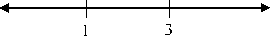
\includegraphics{images/image109.png}
\caption{}
\end{figure}

We already know the derivative is zero or undefined at the critical
numbers. On each interval between these values, the derivative will stay
the same sign. To determine the sign, we could pick a test value in each
interval, and evaluate the derivative at those points (or use the sign
approach used above).

\begin{figure}
\centering
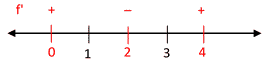
\includegraphics{images/image110.png}
\caption{}
\end{figure}

At (3, 2) \textbackslash{}(f'\textbackslash{}) changes from negative to
positive, so there is a local min at (3, 2). This confirms what we saw
before in the graph.

\begin{figure}
\centering
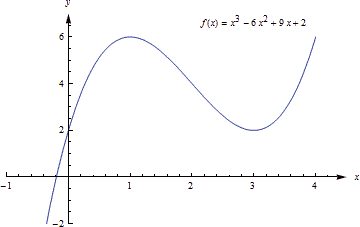
\includegraphics{images/image058.png}
\caption{}
\end{figure}

To view this video please enable JavaScript, and consider upgrading to a
web browser that \href{http://videojs.com/html5-video-support/}{supports
HTML5 video}

To view this video please enable JavaScript, and consider upgrading to a
web browser that \href{http://videojs.com/html5-video-support/}{supports
HTML5 video}

\hypertarget{f-and-extreme-values-of-f-1}{%
\subsubsection{\textbackslash{}(f''\textbackslash{}) and Extreme Values
of
\textbackslash{}(f\textbackslash{})}\label{f-and-extreme-values-of-f-1}}

The concavity of a function can also help us determine whether a
critical point is a maximum or minimum or neither. For example, if a
point is at the bottom of a concave up function, then the point is a
minimum.

\begin{figure}
\centering
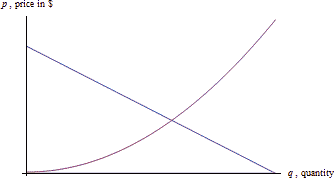
\includegraphics{images/image062.png}
\caption{}
\end{figure}

\hypertarget{the-second-derivative-test-for-extremes}{%
\paragraph{The Second Derivative Test for
Extremes}\label{the-second-derivative-test-for-extremes}}

Find all critical points of \textbackslash{}(f\textbackslash{}). For
those critical points where \textbackslash{}(f'(c) = 0\textbackslash{}),
find \textbackslash{}(f''(c)\textbackslash{}).

\begin{itemize}
\tightlist
\item
  If \textbackslash{}(f''(c) \textbackslash{}lt 0\textbackslash{})
  (negative) then \textbackslash{}(f\textbackslash{}) is concave down
  and has a local maximum at \textbackslash{}(x = c\textbackslash{}).
\item
  If \textbackslash{}(f''(c) \textbackslash{}gt 0\textbackslash{})
  (positive) then \textbackslash{}(f\textbackslash{}) is concave up and
  has a local minimum at \textbackslash{}(x = c\textbackslash{}).
\item
  If \textbackslash{}(f''(c) = 0\textbackslash{}) then
  \textbackslash{}(f\textbackslash{}) may have a local maximum, a
  minimum or neither at \textbackslash{}(x = c\textbackslash{}).
\end{itemize}

The cartoon faces can help you remember the Second Derivative Test.

\begin{figure}
\centering
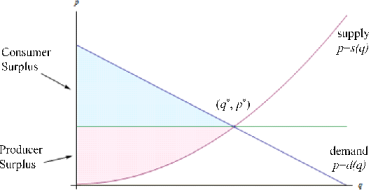
\includegraphics{images/image063.png}
\caption{}
\end{figure}

\hypertarget{example-5}{%
\paragraph{Example 5}\label{example-5}}

\textbackslash{}(f(x) = 2x\^{}3 - 15x\^{}2 + 24x - 7\textbackslash{})
has critical numbers \textbackslash{}(x =\textbackslash{}) 1 and 4. Use
the Second Derivative Test for Extremes to determine whether
\textbackslash{}(f(1)\textbackslash{}) and
\textbackslash{}(f(4)\textbackslash{}) are maximums or minimums or
neither.

We need to find the second derivative: \textbackslash{}{[}
\textbackslash{}begin\{align*\} f(x)=\& 2x\^{}3 - 15x\^{}2 + 24x -
7\textbackslash{}\textbackslash{} f'(x)=\& 6x\^{}2 - 30x +
24\textbackslash{}\textbackslash{} f''(x)=\& 12x - 30
\textbackslash{}end\{align*\} \textbackslash{}{]}

Then we just need to evaluate \textbackslash{}(f''\textbackslash{}) at
each critical number:

\textbackslash{}(x = 1\textbackslash{}): \textbackslash{}(
f''(1)=12(1)-30 \textbackslash{}lt 0 \textbackslash{}), so there is a
local maximum at \textbackslash{}(x = 1\textbackslash{}).

\textbackslash{}(x = 4\textbackslash{}): \textbackslash{}(
f''(4)=12(4)-30 \textbackslash{}gt 0 \textbackslash{}), so there is a
local minimum at \textbackslash{}(x = 4\textbackslash{}).

To view this video please enable JavaScript, and consider upgrading to a
web browser that \href{http://videojs.com/html5-video-support/}{supports
HTML5 video}

Many students like the Second Derivative Test. The Second Derivative
Test is often easier to use than the First Derivative Test. You only
have to find the sign of one number for each critical number rather than
two. And if your function is a polynomial, its second derivative will
probably be a simpler function than the derivative.

However, if you needed a product rule, quotient rule, or chain rule to
find the first derivative, finding the second derivative can be a lot of
work. Also, even if the second derivative is easy, the Second Derivative
Test doesn't always give an answer. The First Derivative Test will
always give you an answer.

Use whichever test you want to. But remember -- you have to do some test
to be sure that your critical point actually is a local max or min.

To view this video please enable JavaScript, and consider upgrading to a
web browser that \href{http://videojs.com/html5-video-support/}{supports
HTML5 video}

To view this video please enable JavaScript, and consider upgrading to a
web browser that \href{http://videojs.com/html5-video-support/}{supports
HTML5 video}

\hypertarget{global-maxima-and-minima}{%
\subsection{Global Maxima and Minima}\label{global-maxima-and-minima}}

In applications, we often want to find the global extreme; knowing that
a critical point is a local extreme is not enough.

For example, if we want to make the greatest profit, we want to make the
absolutely greatest profit of all. How do we find global max and min?

There are just a few additional things to think about.

\hypertarget{endpoint-extremes}{%
\subsubsection{Endpoint Extremes}\label{endpoint-extremes}}

The local extremes of a function occur at critical points -- these are
points in the function that we can find by thinking about the shape (and
using the derivative to help us). But if we're looking at a function on
a closed interval, the endpoints could be extremes. These endpoint
extremes are not related to the shape of the function; they have to do
with the interval, the window through which we're viewing the function.

\begin{figure}
\centering
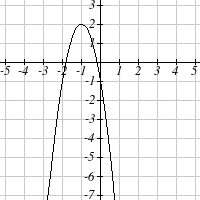
\includegraphics{images/image064.png}
\caption{}
\end{figure}

In the graph above, it appears that there are three critical points --
one local min, one local max, and one that is neither one. But the
global max, the highest point of all, is at the left endpoint. The
global min, the lowest point of all, is at the right endpoint.

How do we decide if endpoints are global max or min? It's easier than
you expected -- simply plug in the endpoints, along with all the
critical numbers, and compare
\textbackslash{}(y\textbackslash{})-values.

\hypertarget{example-6}{%
\paragraph{Example 6}\label{example-6}}

Find the global max and min of \textbackslash{}(f(x) = x\^{}3 - 3x\^{}2
- 9x + 5\textbackslash{}) for \textbackslash{}(-2 \textbackslash{}leq x
\textbackslash{}leq 6\textbackslash{}).

\textbackslash{}(f'(x) = 3x\^{}2 - 6x - 9 = 3(x + 1)(x -
3)\textbackslash{}). We need to find critical points, and we need to
check the endpoints.

\textbackslash{}(f'(x) = 3(x + 1)(x - 3) = 0\textbackslash{}) when
\textbackslash{}(x = -1\textbackslash{}) and \textbackslash{}(x =
3\textbackslash{}). The endpoints of the interval are \textbackslash{}(x
= -2\textbackslash{}) and \textbackslash{}(x = 6\textbackslash{}).

Now we simply compare the values of \textbackslash{}(f\textbackslash{})
at these four values of \textbackslash{}(x\textbackslash{}):

\begin{longtable}[]{@{}ll@{}}
\toprule
\endhead
\textbackslash{}( x \textbackslash{}) & \textbackslash{}( f(x)
\textbackslash{})\tabularnewline
-2 & 3\tabularnewline
-1 & 10\tabularnewline
3 & -22\tabularnewline
6 & 59\tabularnewline
\bottomrule
\end{longtable}

The global minimum of \textbackslash{}(f\textbackslash{}) on
\textbackslash{}({[} -2, 6{]}\textbackslash{}) is -22, when
\textbackslash{}(x = 3\textbackslash{}), and the global maximum of
\textbackslash{}(f\textbackslash{}) on \textbackslash{}({[} -2,
6{]}\textbackslash{}) is 59, when \textbackslash{}(x =
6\textbackslash{}).

To view this video please enable JavaScript, and consider upgrading to a
web browser that \href{http://videojs.com/html5-video-support/}{supports
HTML5 video}

\hypertarget{if-theres-only-one-critical-point}{%
\subsubsection{If there's only one critical
point}\label{if-theres-only-one-critical-point}}

If the function has only one critical point and it's a local max (or
min), then it must be the global max (or min). To see this, think about
the geometry. Look at the graph on the left -- there is a local max, and
the graph goes down on either side of the critical point. Suppose there
was some other point that was higher -- then the graph would have to
turn around. But that turning point would have shown up as another
critical point. If there's only one critical point, then the graph can
never turn back around.

\begin{figure}
\centering
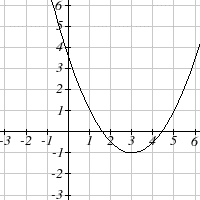
\includegraphics{images/image065.png}
\caption{}
\end{figure}

\hypertarget{when-in-doubt-graph-it-and-look.}{%
\subsubsection{When in doubt, graph it and
look.}\label{when-in-doubt-graph-it-and-look.}}

If you are trying to find a global max or min on an open interval (or
the whole real line), and there is more than one critical point, then
you need to look at the graph to decide whether there is a global max or
min. Be sure that all your critical points show in your graph, and that
you graph beyond them -- that will tell you what you want to know.

\hypertarget{example-7}{%
\paragraph{Example 7}\label{example-7}}

Find the global max and min of \textbackslash{}(f(x) = x\^{}3 - 6x\^{}2
+ 9x + 2\textbackslash{}).

We have previously found that (1, 6) is a local max and (3, 2) is a
local min. This is not a closed interval, and there are two critical
points, so we must turn to the graph of the function to find global max
and min.

The graph of \textbackslash{}(f\textbackslash{}) shows that points to
the left of \textbackslash{}(x = 4\textbackslash{}) have
\textbackslash{}(y\textbackslash{})-values greater than 6, so (1, 6) is
not a global max. Likewise, if \textbackslash{}(x\textbackslash{}) is
negative, \textbackslash{}(y\textbackslash{}) is less than 2, so (3, 2)
is not a global min. There are no endpoints, so we've exhausted all the
possibilities. This function does not have a global maximum or minimum.

\begin{figure}
\centering
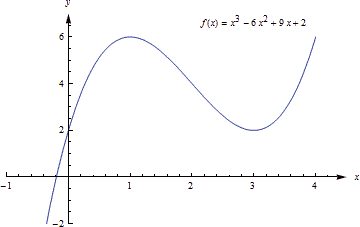
\includegraphics{images/image058.png}
\caption{}
\end{figure}

\hypertarget{to-find-global-extremes}{%
\paragraph{To find Global Extremes}\label{to-find-global-extremes}}

The only places where a function can have a global extreme are critical
points or endpoints.

\begin{itemize}
\tightlist
\item
  If the function has only one critical point, and it's a local extreme,
  then it is also the global extreme.
\item
  If there are endpoints, find the global extremes by comparing
  \textbackslash{}(y\textbackslash{})-values at all the critical points
  and at the endpoints.
\item
  When in doubt, graph the function to be sure. (However, unless the
  problem explicitly tells you otherwise, it is \textbf{not} enough to
  just use the graph to get your answer.)
\end{itemize}

\begin{longtable}[]{@{}ll@{}}
\toprule
\endhead
\href{section2-6.php}{← Previous Section} & \href{section2-8.php}{Next
Section →}\tabularnewline
\bottomrule
\end{longtable}
